\mfpicnumber{1}

\opengraphsfile{MatMethods}

\setcounter{footnote}{0}

\label{MatMethods}

\setlength{\extrarowheight}{0pt}

We concluded Section \ref{MatArithmetic} by showing how we can rewrite a system of linear equations as the matrix equation $AX=B$ where $A$ and $B$ are known matrices and the solution matrix $X$ of the equation corresponds to the solution of the system. In this section, we develop the method for solving such an equation.  To that end, consider the system \[ \left\{ \begin{array}{rcr} 2x-3y & = & 16 \\ 3x+4y & = & 7 \\ \end{array} \right.\]  To write this as a matrix equation, we follow the procedure outlined on page \pageref{systemasmatrixeqn}.  We find the coefficient matrix $A$, the unknowns matrix $X$ and constant matrix $B$ to be 
\[ \begin{array}{ccc} 

A = \left[ \begin{array}{rr} 2 & -3 \\ 3 & 4 \\ \end{array} \right] 

&

 X = \left[ \begin{array}{r} x \\ y \\ \end{array} \right]
 
&

 B = \left[ \begin{array}{r} 16 \\ 7 \\ \end{array} \right] 
 \end{array}\]   
 
In order to motivate how we solve a matrix equation like $AX = B$, we revisit solving a similar equation involving real numbers. For instance, to solve  $3x = 5$,  we  divide both sides by $3$ and obtain $x = \frac{5}{3}$.  How can we go about defining an analogous process for matrices? To answer this question, we solve $3x=5$ again, but this time, we pay attention to the properties of real numbers being used at each step.  Recall that dividing by $3$ is the same as multiplying by $\frac{1}{3} = 3^{-1}$, the so-called \textit{multiplicative inverse}\footnote{Every nonzero real number $a$ has a multiplicative inverse, denoted $a^{-1}$, such that  $a^{-1} \cdot a = a \cdot a^{-1} = 1$.} of $3$.


\[ \begin{array}{rclr}

3x & = & 5 \\
3^{-1}(3x) & = & 3^{-1}(5) & \text{Multiply by the (multiplicative) inverse of $3$} \\
\left(3^{-1}\cdot 3\right) x & = & 3^{-1}(5) & \text{Associative property of multiplication} \\
1 \cdot x &  = & 3^{-1}(5) & \text{Inverse property} \\
 x &  = & 3^{-1}(5) & \text{Multiplicative Identity} \\
 
\end{array} \]

If we wish to check our answer, we substitute $x = 3^{-1}(5)$ into the original equation

\[ \begin{array}{rclr}

3x & \stackrel{?}{=} & 5 \\
3\left( 3^{-1}(5)\right) & \stackrel{?}{=} & 5 \\
\left(3 \cdot 3^{-1}\right)(5) & \stackrel{?}{=} & 5 & \text{Associative property of multiplication}  \\
1 \cdot 5 & \stackrel{?}{=} & 5 & \text{Inverse property} \\
5 & \stackrel{\checkmark}{=} & 5 & \text{Multiplicative Identity} \\
\end{array} \]

Thinking back to Theorem \ref{matrixmultprops}, we know that matrix multiplication enjoys both an associative property and a multiplicative identity.  What's missing from the mix is a multiplicative inverse for the coefficient matrix $A$.  Assuming we can find such a beast, we can mimic our solution (and check) to $3x=5$ as follows

\[ \begin{array}{cc}  

\text{Solving $AX = B$} & \text{Checking our answer} \\

\begin{array}{rcl}

AX & = & B \\

A^{-1}(AX) & = & A^{-1}B \\

\left(A^{-1}A\right) X & = & A^{-1}B \\

I_{\mbox{\tiny$2$}}X & = & A^{-1}B \\

X & = & A^{-1}B \\

\end{array} 

&

\begin{array}{rcl}

AX & \stackrel{?}{=} & B \\

A \left(A^{-1}B\right) & \stackrel{?}{=} & B \\

\left(AA^{-1}\right) B & \stackrel{?}{=}& B \\

I_{\mbox{\tiny$2$}}B & \stackrel{?}{=} & B \\

B & \stackrel{\checkmark}{=}& B \\

\end{array} \\

\end{array}\]

\phantomsection \label{solvingmatrixeqn}

The matrix $A^{-1}$ is read `$A$-inverse' and we will define it formally later in the section. At this stage, we have no idea if such a matrix $A^{-1}$ exists, but that won't deter us from trying to find it.\footnote{Much like Carl's quest to find Sasquatch.} 

We want $A^{-1}$ to satisfy two equations, $A^{-1}A = I_{\mbox{\tiny$2$}}$ and $AA^{-1} = I_{\mbox{\tiny$2$}}$, making $A^{-1}$ necessarily a $2 \times 2$ matrix.\footnote{Since matrix multiplication isn't necessarily commutative, at this stage, these are two different equations.}  Hence,  $A^{-1}$ has the form 

\[  A^{-1} = \left[ \begin{array}{rr} x_{\mbox{\tiny$1$}} & x_{\mbox{\tiny$2$}} \\ x_{\mbox{\tiny$3$}} & x_{\mbox{\tiny$4$}} \\ \end{array} \right]\]

for real numbers $x_{\mbox{\tiny$1$}}$, $x_{\mbox{\tiny$2$}}$, $x_{\mbox{\tiny$3$}}$ and $x_{\mbox{\tiny$4$}}$.  For reasons which will become clear later, we focus our attention on the equation $AA^{-1} = I_{\mbox{\tiny$2$}}$.  We have

\[\begin{array}{rcl}

AA^{-1} & = & I_{2} \\ [13pt]

\left[ \begin{array}{rr} 2 & -3 \\ 3 & 4 \\ \end{array} \right] \left[ \begin{array}{rr} x_{\mbox{\tiny$1$}} & x_{\mbox{\tiny$2$}} \\ x_{\mbox{\tiny$3$}} & x_{\mbox{\tiny$4$}} \\ \end{array} \right]  & = & \left[ \begin{array}{rr} 1 & 0 \\ 0 & 1 \\ \end{array} \right] \\ [13pt]

\left[ \begin{array}{rr} 2x_{\mbox{\tiny$1$}} - 3x_{\mbox{\tiny$3$}} &  2x_{\mbox{\tiny$2$}} - 3x_{\mbox{\tiny$4$}} \\ 3x_{\mbox{\tiny$1$}} +4x_{\mbox{\tiny$3$}} &  3x_{\mbox{\tiny$2$}} +4x_{\mbox{\tiny$4$}} \\ \end{array} \right]  & = & \left[ \begin{array}{rr} 1 & 0 \\ 0 & 1 \\ \end{array} \right] \\

\end{array} \] 

This gives rise to \textit{two} more systems of equations

\[\begin{array}{cc}

\left\{ \begin{array}{rcr} 2x_{\mbox{\tiny$1$}}-3x_{\mbox{\tiny$3$}} & = & 1 \\ 3x_{\mbox{\tiny$1$}}+4x_{\mbox{\tiny$3$}} & = & 0 \\ \end{array} \right.

&

\left\{ \begin{array}{rcr} 2x_{\mbox{\tiny$2$}}-3x_{\mbox{\tiny$4$}} & = & 0 \\ 3x_{\mbox{\tiny$2$}}+4x_{\mbox{\tiny$4$}} & = & 1 \\ \end{array} \right.

\end{array}\]

At this point, it may seem absurd to continue with this venture.  After all, the intent was to solve \textit{one} system of equations, and in doing so, we have produced \textit{two} more to solve.  Remember, the objective of this discussion is to develop a general \textit{method} which, when used in the correct scenarios, allows us to do far more than just solve a system of equations. 

 If we set about solving these systems using augmented matrices using the techniques in Section \ref{AugMatrices}, we see that not only do both systems have the same coefficient matrix, this coefficient matrix is none other than the matrix $A$ itself!  (We will come back to this observation in a moment.)  

\[ \begin{array}{ccc}

\left\{ \begin{array}{rcr} 2x_{\mbox{\tiny$1$}}-3x_{\mbox{\tiny$3$}} & = & 1 \\ 3x_{\mbox{\tiny$1$}}+4x_{\mbox{\tiny$3$}} & = & 0 \\ \end{array} \right.

&
\xrightarrow{\text{Encode into a matrix}}

&
\left[ \begin{array}{rr|r} 2 & -3 & 1 \\ 3 & 4 & 0 \\ \end{array} \right] \\ [13pt]


\left\{ \begin{array}{rcr} 2x_{\mbox{\tiny$2$}}-3x_{\mbox{\tiny$4$}} & = & 0 \\ 3x_{\mbox{\tiny$2$}}+4x_{\mbox{\tiny$4$}} & = & 1 \\ \end{array} \right. 

&
\xrightarrow{\text{Encode into a matrix}}

&

\left[ \begin{array}{rr|r} 2 & -3 & 0 \\ 3 & 4 & 1 \\ \end{array} \right] \\

\end{array} \]

To solve these two systems, we use Gauss-Jordan Elimination to put the augmented matrices into reduced row echelon form. (We leave the details to the reader.) For the first system, we get 

\[ \begin{array}{ccc}

\left[ \begin{array}{rr|r} 2 & -3 & 1 \\ 3 & 4 & 0 \\ \end{array} \right] 
&
\xrightarrow{\text{Gauss Jordan Elimination}}

&
\left[ \begin{array}{rr|r} 1 & 0 & \frac{4}{17} \\[3pt] 0 & 1 & -\frac{3}{17} \\ \end{array} \right] \\

\end{array}\]

which gives $x_{\mbox{\tiny$1$}} =  \frac{4}{17}$ and $x_{\mbox{\tiny$3$}} = -\frac{3}{17}$.  To solve the second system, we use the exact same row operations, in the same order, and we obtain

\[ \begin{array}{ccc}

\left[ \begin{array}{rr|r} 2 & -3 & 0 \\ 3 & 4 & 1 \\ \end{array} \right] 
&
\xrightarrow{\text{Gauss Jordan Elimination}}

&
\left[ \begin{array}{rr|r} 1 & 0 & \frac{3}{17} \\[3pt] 0 & 1 & \frac{2}{17} \\ \end{array} \right] \\

\end{array}\]

which means $x_{\mbox{\tiny$2$}} = \frac{3}{17}$ and $x_{\mbox{\tiny$4$}} = \frac{2}{17}$.  Hence, 

\[  A^{-1} = \left[ \begin{array}{rr} x_{\mbox{\tiny$1$}} & x_{\mbox{\tiny$2$}} \\ x_{\mbox{\tiny$3$}} & x_{\mbox{\tiny$4$}} \\ \end{array} \right] = \left[ \begin{array}{rr} \frac{4}{17} & \frac{3}{17} \\[3pt]  -\frac{3}{17} & \frac{2}{17} \\ \end{array} \right]   \]

We can check to see that $A^{-1}$ behaves as it should by computing $AA^{-1}$

\[ AA^{-1} = \left[ \begin{array}{rr} 2 & -3 \\ 3 & 4 \\ \end{array} \right] \left[ \begin{array}{rr} \frac{4}{17} & \frac{3}{17} \\[3pt]  -\frac{3}{17} & \frac{2}{17} \\ \end{array} \right] = \left[ \begin{array}{rr} 1 & 0 \\ 0 & 1 \\ \end{array} \right] = I_{\mbox{\tiny$2$}} \, \, \checkmark\]

As an added bonus, 

\[ A^{-1}A = \left[ \begin{array}{rr} \frac{4}{17} & \frac{3}{17} \\[3pt]  -\frac{3}{17} & \frac{2}{17} \\ \end{array} \right]\left[ \begin{array}{rr} 2 & -3 \\ 3 & 4 \\ \end{array} \right]  = \left[ \begin{array}{rr} 1 & 0 \\ 0 & 1 \\ \end{array} \right] = I_{\mbox{\tiny$2$}} \, \, \checkmark\]

We can now return to the problem at hand.  From our discussion  on page \pageref{solvingmatrixeqn}, we know

\[ X = A^{-1}B = \left[ \begin{array}{rr} \frac{4}{17} & \frac{3}{17} \\[3pt]  -\frac{3}{17} & \frac{2}{17} \\ \end{array} \right]\left[ \begin{array}{r} 16 \\ 7 \\ \end{array} \right] = \left[ \begin{array}{r} 5 \\ -2 \\ \end{array} \right] \]

so that our final solution to the system is $(x,y) = (5,-2)$.   

\smallskip

As mentioned, the point of this exercise was not just to solve the system of linear equations, but to develop a general method for finding $A^{-1}$.  To that end, we analyze the foregoing discussion in a more general context. To find $A^{-1}$, we used two augmented matrices, both containing the entries as $A$:

\[ \begin{array}{rcl}

\left[ \begin{array}{rr|r} 2 & -3 & 1 \\ 3 & 4 & 0 \\ \end{array} \right] & = & \left[ \begin{tabular}{c|r}
\multirow{2}{10pt}{\large \textit{A}} & 1 \\ & 0 \end{tabular} \right] \\ [13pt]

\left[ \begin{array}{rr|r} 2 & -3 & 0 \\ 3 & 4 & 1 \\ \end{array} \right] & = & \left[ \begin{tabular}{c|r} \multirow{2}{10pt}{\large \textit{A}} & 0 \\ & 1 \end{tabular} \right] \\ [13pt]

\end{array} \]

We also note that the reduced row echelon forms of these augmented matrices can be written as

\[ \begin{array}{rcl}

\left[ \begin{array}{rr|r} 1 & 0 & \frac{4}{17} \\[3pt] 0 & 1 & -\frac{3}{17} \\ \end{array} \right] & = & \left[ \begin{tabular}{c|r} \multirow{2}{10pt}{\large $I_{\mbox{\tiny$2$}}$} & $x_{\mbox{\tiny$1$}}$ \\[3pt] &  $x_{\mbox{\tiny$3$}}$ \end{tabular} \right]\\ [13pt]

\left[ \begin{array}{rr|r} 1 & 0 & \hphantom{-}\frac{3}{17} \\[3pt] 0 & 1 & \frac{2}{17} \\ \end{array} \right] & = & \left[ \begin{tabular}{c|r} \multirow{2}{10pt}{\large $I_{\mbox{\tiny$2$}}$} & $x_{\mbox{\tiny$2$}}$ \\[3pt] & $x_{\mbox{\tiny$4$}}$ \end{tabular} \right]

\end{array} \]

where we have identified the entries to the left of the vertical bar as the identity $I_{\mbox{\tiny$2$}}$ and the entries to the right of the vertical bar as the solutions to our systems.  The long and short of the solution process can be summarized as

\[ \begin{array}{ccc}

\left[ \begin{tabular}{c|r} \multirow{2}{10pt}{\large \textit{A}} & 1 \\ & 0 \end{tabular} \right]
&
\xrightarrow{\text{Gauss Jordan Elimination}}
&
\left[ \begin{tabular}{c|r} \multirow{2}{10pt}{\large $I_{\mbox{\tiny$2$}}$} & $x_{\mbox{\tiny$1$}}$ \\ &  $x_{\mbox{\tiny$3$}}$ \end{tabular} \right]  \\ [13pt]

\left[ \begin{tabular}{c|r} \multirow{2}{10pt}{\large \textit{A}} & 0 \\ & 1 \end{tabular} \right]
&
\xrightarrow{\text{Gauss Jordan Elimination}}
&
\left[ \begin{tabular}{c|r} \multirow{2}{10pt}{\large $I_{\mbox{\tiny$2$}}$} & $x_{\mbox{\tiny$2$}}$ \\ & $x_{\mbox{\tiny$4$}}$ \end{tabular} \right]

\end{array}\]

Since the row operations for both processes are the same, all of the arithmetic on the left hand side of the vertical bar is identical in both problems.  The only difference between the two processes is what happens to the constants to the right of the vertical bar.  As long as we keep these separated into columns, we can combine our efforts into one `super-sized' augmented matrix and describe the above process as

\[ \begin{array}{ccc}

\left[ \begin{tabular}{c|rr} \multirow{2}{10pt}{\large \textit{A}} & 1 & 0 \\ & 0 & 1 \end{tabular} \right]
&
\xrightarrow{\text{Gauss Jordan Elimination}}
&
\left[ \begin{tabular}{c|rr} \multirow{2}{10pt}{\large $I_{\mbox{\tiny$2$}}$} & $x_{\mbox{\tiny$1$}}$ & $x_{\mbox{\tiny$2$}}$ \\ &  $x_{\mbox{\tiny$3$}}$ & $x_{\mbox{\tiny$4$}}$ \end{tabular} \right]

\end{array}\]

We have the identity matrix $I_{\mbox{\tiny$2$}}$ appearing as the right hand side of the first super-sized augmented matrix and the left hand side of the second super-sized augmented matrix.  To our surprise and delight, the elements on the right hand side of the second super-sized augmented matrix are none other than those which comprise $A^{-1}$.  Hence, we have

\[ \begin{array}{ccc}

\left[ \begin{array}{c|c} A & I_{\mbox{\tiny$2$}} \end{array} \right]

&
\xrightarrow{\text{Gauss Jordan Elimination}}

&

\left[ \begin{array}{c|c} I_{\mbox{\tiny$2$}} & A^{-1} \end{array} \right] 

\end{array}\]

In other words, the process of finding $A^{-1}$ for a matrix $A$ can be viewed as performing a series of row operations which transform $A$ into the identity matrix of the same dimension.  We can view this process as follows.  In trying to find $A^{-1}$, we are trying to `undo' multiplication by the matrix $A$.  The identity matrix in the  super-sized augmented matrix $[A | I]$ keeps a running memory of all of the moves required to `undo' $A$. This results in exactly what we want, $A^{-1}$.  We are now ready to formalize and generalize the foregoing discussion.  We begin with the formal definition of an invertible matrix.\footnote{If this rhetoric sounds familiar, it should. See section \ref{InverseFunctions}.} 

\smallskip

\colorbox{ResultColor}{\bbm

\begin{defn}  \label{matrixinverse}  An $n \times n$ matrix $A$ is said to be \index{matrix ! invertible}\index{matrix ! multiplicative inverse}\index{invertible ! matrix}\textbf{invertible} if there exists a matrix $A^{-1}$, read `$A$ inverse', such that $A^{-1}A = AA^{-1}=I_{n}$. \index{inverse ! matrix, multiplicative}
\end{defn}
\ebm}


\smallskip

Note that, as a consequence of our definition, invertible matrices are square, and as such, the conditions in Definition \ref{matrixinverse} force the matrix $A^{-1}$ to be same dimensions as $A$, that is, $n \times n$.  Since not all matrices are square, not all matrices are invertible.  However, just because a matrix is square doesn't guarantee it is invertible.  (See the exercises.)   

Our first result summarizes some of the important characteristics of invertible matrices and their inverses.  

\smallskip

\colorbox{ResultColor}{\bbm

\begin{thm}  \label{inversematrixprops}  Suppose $A$ is an $n \times n$ matrix. 


\vspace{-.1in} 

\begin{enumerate}

\item  If $A$ is invertible then $A^{-1}$ is unique.

\vspace{-.1in}

\item  $A$ is invertible if and only if $AX = B$ has a unique solution for every $n \times r$ matrix $B$.  

\end{enumerate}

\end{thm}

\ebm}

\smallskip

The proofs of the properties in Theorem \ref{inversematrixprops} rely on a healthy mix of definition and matrix arithmetic.  

To establish the first property, we assume that $A$ is invertible and suppose the matrices $B$ and $C$ act as inverses for $A$.  That is, $BA = AB = I_{n}$ and $CA = AC = I_{n}$.  We need to show that $B$ and $C$ are, in fact, the same matrix.  To see this, we note that $B = I_{n}B = (CA)B = C(AB) = CI_{n} = C$. Hence, any two matrices that act like $A^{-1}$ are, in fact, the same matrix.\footnote{If this proof sounds familiar, it should. See the discussion following Theorem \ref{inversefunctionprops}.}  

To prove the second property of Theorem  \ref{inversematrixprops}, we note that if $A$ is invertible then the discussion on page \pageref{solvingmatrixeqn} shows the solution to $AX=B$ to be $X = A^{-1}B$, and since $A^{-1}$ is unique, so is $A^{-1}B$. 

Conversely, if $AX = B$ has a unique solution for every $n \times r$ matrix $B$, then, in particular, there is a unique solution $X_{0}$ to the equation $AX = I_{n}$.  The solution matrix $X_{0}$ is our candidate for $A^{-1}$. We have $AX_{0} = I_{n}$ by definition, but we need to also show $X_{0}A = I_{n}$.  To that end, we note that $A\left(X_{0}A\right) = \left(AX_{0}\right)A = I_{n}A = A$.  In other words, the matrix $X_{0}A$ is a solution to the equation $AX = A$.  Clearly, $X=I_{n}$ is also a solution to the equation $AX = A$, and since we are assuming every such equation as a \textit{unique} solution, we must have $X_{0}A = I_{n}$.  Hence, we have $X_{0}A = AX_{0} = I_{n}$, so that $X_{0} = A^{-1}$ and $A$ is invertible.  

The foregoing discussion justifies our quest to find $A^{-1}$ using our super-sized augmented matrix approach
 
\[ \begin{array}{ccc}

\left[ \begin{array}{c|c} A & I_{n} \\ \end{array} \right]

&
\xrightarrow{\text{Gauss Jordan Elimination}}

&

\left[ \begin{array}{c|c} I_{n} & A^{-1} \\ \end{array} \right] 

\end{array}\]

We are, in essence, trying to find the unique solution to the equation $AX = I_{n}$ using row operations.

\smallskip

What does all of this mean for a system of linear equations?  Theorem \ref{inversematrixprops} tells us that if we write the system in the form $AX=B$, then if the coefficient matrix $A$ is invertible, there is only one solution to the system $-$ that is, if $A$ is invertible, the system is consistent and independent.\footnote{It can be shown that a matrix is invertible if and only if when it serves as a coefficient matrix for a system of equations, the system is always consistent independent. It amounts to the second property in Theorem \ref{inversematrixprops} where the matrices $B$ are restricted to being $n \times 1$ matrices.  We note that, owing to how matrix multiplication is defined, being able to find unique solutions to $AX = B$ for $n \times 1$ matrices $B$ gives you the same statement about solving such equations for $n \times r$ matrices $-$ since we can find a unique solution to them one column at a time.}  

We also know that the process by which we find $A^{-1}$ is determined completely by $A$, and not by the constants in $B$.  This answers the question as to why we would bother doing row operations on a super-sized augmented matrix to find $A^{-1}$ instead of an ordinary augmented matrix to solve a system;  by finding $A^{-1}$ we have done all of the row operations we ever need to do, once and for all, since we can quickly solve \textit{any} equation $AX = B$ using \textit{one} multiplication, $A^{-1}B$.

\begin{ex} \label{matrixinverseex} Let $A = \left[ \begin{array}{rrr} 3 & 1 & \hphantom{-}2 \\ 0 & -1 & 5 \\ 2 & 1 & 4 \\ \end{array} \right]$

\begin{enumerate}

\item  Use row operations to find $A^{-1}$.  Check your answer by finding $A^{-1}A$ and $AA^{-1}$.

\item  Use $A^{-1}$ to solve the following systems of equations

\begin{multicols}{3}

\begin{enumerate}

\item $\left\{ \begin{array}{rcl}   3x+y+2z & = & 26 \\-y+5z & = & 39 \\ 2x+y+4z&=& 117 \\ \end{array} \right.$

\item $\left\{ \begin{array}{rcl} 3x+y+2z & = & 4 \\-y+5z & = & 2 \\ 2x+y+4z&=& 5 \\ \end{array} \right.$

\item $\left\{ \begin{array}{rcl} 3x+y+2z & = & 1 \\-y+5z & = & 0 \\ 2x+y+4z&=& 0 \\ \end{array} \right.$

\end{enumerate}

\end{multicols}

\end{enumerate}

{\bf Solution.}  

\begin{enumerate}

\item  We begin with a super-sized augmented matrix and proceed with Gauss-Jordan elimination.

\begin{flushleft}

$\begin{array}{ccc}

\left[ \begin{array}{rrr|rrr} 3 & 1 & \hphantom{-}2 & 1 & 0 & 0 \\ 0 & -1 & 5 & 0 & 1 & 0 \\ 2 & 1 & 4 & 0 & 0 & 1 \\ \end{array} \right]

&

\xrightarrow[\text{with $\frac{1}{3}R1$}]{\text{Replace $R1$}}

&

\left[ \begin{array}{rrr|rrr} 1 & \frac{1}{3} & \hphantom{-}\frac{2}{3} & \frac{1}{3} & 0 & 0 \\ 0 & -1 & 5 & 0 & 1 & 0 \\ 2 & 1 & 4 & 0 & 0 & 1 \\ \end{array} \right]

\end{array}$

$\begin{array}{ccc}

\left[ \begin{array}{rrr|rrr} 1 & \frac{1}{3} & \hphantom{-}\frac{2}{3} & \frac{1}{3} & 0 & 0 \\ 0 & -1 & 5 & 0 & 1 & 0 \\ 2 & 1 & 4 & 0 & 0 & 1 \\ \end{array} \right]

\xrightarrow[\text{$-2R1+R3$}]{\text{Replace $R3$ with}}  

\left[ \begin{array}{rrr|rrr} 1 & \frac{1}{3} & \hphantom{-}\frac{2}{3} & \frac{1}{3} & 0 & 0 \\ 0 & -1 & 5 & 0 & 1 & 0 \\ 0 & \frac{1}{3} & \frac{8}{3} & -\frac{2}{3} & 0 & 1 \\ \end{array} \right]

\end{array}$

$\begin{array}{ccc}

\left[ \begin{array}{rrr|rrr} 1 & \frac{1}{3} & \hphantom{-}\frac{2}{3} & \frac{1}{3} & 0 & 0 \\ 0 & -1 & 5 & 0 & 1 & 0 \\ 0 & \frac{1}{3} & \frac{8}{3} & -\frac{2}{3} & 0 & 1 \\ \end{array} \right]

&

\xrightarrow[\text{with $(-1)R2$}]{\text{Replace $R2$}}

&

\left[ \begin{array}{rrr|rrr} 1 & \hphantom{-}\frac{1}{3} & \frac{2}{3} & \frac{1}{3} & 0 & \hphantom{-}0 \\ 0 & 1 & -5 & 0 & -1 & 0 \\ 0 & \frac{1}{3} & \frac{8}{3} & -\frac{2}{3} & 0 & 1 \\ \end{array} \right]

\end{array}$

$\begin{array}{ccc}

\left[ \begin{array}{rrr|rrr} 1 & \hphantom{-}\frac{1}{3} & \frac{2}{3} & \frac{1}{3} & 0 & \hphantom{-}0 \\ 0 & 1 & -5 & 0 & -1 & 0 \\ 0 & \frac{1}{3} & \frac{8}{3} & -\frac{2}{3} & 0 & 1 \\ \end{array} \right]

\xrightarrow[\text{$-\frac{1}{3}R2+R3$}]{\text{Replace $R3$ with}}  

\left[ \begin{array}{rrr|rrr} 1 & \hphantom{-}\frac{1}{3} & \frac{2}{3} & \frac{1}{3} & 0 & \hphantom{-}0 \\ 0 & 1 & -5 & 0 & -1 & 0 \\ 0 & 0 & \frac{13}{3} & -\frac{2}{3} & \frac{1}{3} & 1 \\ \end{array} \right]

\end{array}$

$\begin{array}{ccc}

\left[ \begin{array}{rrr|rrr} 1 & \hphantom{-}\frac{1}{3} & \frac{2}{3} & \frac{1}{3} & 0 & \hphantom{-}0 \\ 0 & 1 & -5 & 0 & -1 & 0 \\ 0 & 0 & \frac{13}{3} & -\frac{2}{3} & \frac{1}{3} & 1 \\ \end{array} \right]

&

\xrightarrow[\text{with $\frac{3}{13}R3$}]{\text{Replace $R3$}}

&

\left[ \begin{array}{rrr|rrr} 1 & \hphantom{-}\frac{1}{3} & \frac{2}{3} & \frac{1}{3} & 0 & 0 \\ 0 & 1 & -5 & 0 & -1 & 0 \\ 0 & 0 & 1 & -\frac{2}{13} & \frac{1}{13} & \frac{3}{13} \\ \end{array} \right]

\end{array}$

$\begin{array}{ccc}

\left[ \begin{array}{rrr|rrr} 1 & \hphantom{-}\frac{1}{3} & \frac{2}{3} & \frac{1}{3} & 0 & 0 \\ 0 & 1 & -5 & 0 & -1 & 0 \\ 0 & 0 & 1 & -\frac{2}{13} & \frac{1}{13} & \frac{3}{13} \\ \end{array} \right]

&

\xrightarrow[\text{\begin{tabular}{c} Replace $R2$ with \\ $5R3+R2$ \end{tabular}}]{\text{\begin{tabular}{c} Replace $R1$ with \\ $-\frac{2}{3}R3+R1$ \end{tabular}}} 

& 

\left[ \begin{array}{rrr|rrr} 1 & \frac{1}{3} & 0 & \frac{17}{39} & -\frac{2}{39} & -\frac{2}{13} \\[3pt] 0 & 1 & 0 &-\frac{10}{13} & -\frac{8}{13} & \frac{15}{13} \\[3pt] 0 & 0 & 1 & -\frac{2}{13} & \frac{1}{13} & \frac{3}{13} \\ \end{array} \right]

\end{array}$

$\begin{array}{ccc}

\left[ \begin{array}{rrr|rrr} 1 & \frac{1}{3} & 0 & \frac{17}{39} & -\frac{2}{39} & -\frac{2}{13} \\[3pt] 0 & 1 & 0 &-\frac{10}{13} & -\frac{8}{13} & \frac{15}{13} \\[3pt] 0 & 0 & 1 & -\frac{2}{13} & \frac{1}{13} & \frac{3}{13} \\ \end{array} \right]
&
\xrightarrow[\text{$-\frac{1}{3}R2+R1$}]{\text{Replace $R1$ with}} 
&

\left[ \begin{array}{rrr|rrr} 1 & 0 & 0 & \frac{9}{13} & \frac{2}{13} & -\frac{7}{13} \\[3pt] 0 & 1 & 0 &-\frac{10}{13} & -\frac{8}{13} & \frac{15}{13} \\[3pt] 0 & 0 & 1 & -\frac{2}{13} & \frac{1}{13} & \frac{3}{13} \\ \end{array} \right]


\end{array}$

\end{flushleft}

We find $A^{-1} = \left[ \begin{array}{rrr} \frac{9}{13} & \frac{2}{13} & -\frac{7}{13} \\[3pt] -\frac{10}{13} & -\frac{8}{13} & \frac{15}{13} \\[3pt] -\frac{2}{13} & \frac{1}{13} & \frac{3}{13} \\ \end{array} \right]$.  To check our answer, we compute

\[ A^{-1}A =  \left[ \begin{array}{rrr} \frac{9}{13} & \frac{2}{13} & -\frac{7}{13} \\[3pt] -\frac{10}{13} & -\frac{8}{13} & \frac{15}{13} \\[3pt] -\frac{2}{13} & \frac{1}{13} & \frac{3}{13}  \end{array} \right]\left[ \begin{array}{rrr} 3 & 1 & \hphantom{-}2 \\[3pt] 0 & -1 & 5 \\[3pt] 2 & 1 & 4 \end{array} \right] = \left[ \begin{array}{rrr} 1 & 0 & 0 \\[3pt] 0 & 1 & 0 \\[3pt] 0 & 0 & 1 \end{array} \right] = I_{3} \, \, \checkmark \]

and 

\[ AA^{-1} = \left[ \begin{array}{rrr} 3 & 1 & \hphantom{-}2 \\[3pt] 0 & -1 & 5 \\[3pt] 2 & 1 & 4  \end{array} \right] \left[ \begin{array}{rrr} \frac{9}{13} & \frac{2}{13} & -\frac{7}{13} \\[3pt] -\frac{10}{13} & -\frac{8}{13} & \frac{15}{13} \\[3pt] -\frac{2}{13} & \frac{1}{13} & \frac{3}{13} \end{array} \right] = \left[ \begin{array}{rrr} 1 & 0 & 0 \\[3pt] 0 & 1 & 0 \\[3pt] 0 & 0 & 1  \end{array} \right] = I_{3} \, \, \checkmark \]

\item Each of the systems in this part has $A$ as its coefficient matrix.  The only difference between the systems is the constants which is the matrix $B$ in the associated matrix equation $AX=B$.  We solve each of them using the formula $X = A^{-1}B$.

\begin{enumerate}

\item $X = A^{-1}B = \left[ \begin{array}{rrr} \frac{9}{13} & \frac{2}{13} & -\frac{7}{13} \\[3pt] -\frac{10}{13} & -\frac{8}{13} & \frac{15}{13} \\[3pt] -\frac{2}{13} & \frac{1}{13} & \frac{3}{13} \end{array} \right] \left[ \begin{array}{r} 26 \\[3pt] 39 \\[3pt] 117 \end{array}\right] =  \left[ \begin{array}{r} -39 \\[3pt] 91 \\[3pt] 26 \end{array}\right]$.  Our solution is $(-39,91,26)$.

\item $X = A^{-1}B = \left[ \begin{array}{rrr} \frac{9}{13} & \frac{2}{13} & -\frac{7}{13} \\[3pt] -\frac{10}{13} & -\frac{8}{13} & \frac{15}{13} \\[3pt] -\frac{2}{13} & \frac{1}{13} & \frac{3}{13}  \end{array} \right] \left[ \begin{array}{r} 4 \\[3pt] 2 \\[3pt] 5 \end{array}\right] =  \left[ \begin{array}{r} \frac{5}{13} \\[3pt] \frac{19}{13} \\[3pt] \frac{9}{13} \end{array}\right]$.  We get $\left( \frac{5}{13},  \frac{19}{13},  \frac{9}{13}   \right)$.

\item $X = A^{-1}B = \left[ \begin{array}{rrr} \frac{9}{13} & \frac{2}{13} & -\frac{7}{13} \\[3pt] -\frac{10}{13} & -\frac{8}{13} & \frac{15}{13} \\[3pt] -\frac{2}{13} & \frac{1}{13} & \frac{3}{13}  \end{array} \right] \left[ \begin{array}{r} 1 \\[3pt] 0 \\[3pt] 0 \end{array}\right] =  \left[ \begin{array}{r} \frac{9}{13} \\[3pt] -\frac{10}{13} \\[3pt] -\frac{2}{13} \end{array}\right]$. We find $\left( \frac{9}{13},  -\frac{10}{13},    -\frac{2}{13}   \right)$.\footnote{Note that the solution is the first column of the $A^{-1}$.  The reader is encouraged to meditate on this `coincidence'.}

\qed

\end{enumerate}

\end{enumerate}

\end{ex}

In Example \ref{matrixinverseex}, we see that finding one inverse matrix can enable us to solve an entire family of systems of linear equations.  There are many examples of where this comes in handy `in the wild', and we chose our example for this section from the field of electronics.  We also take this opportunity to introduce the student to how we can compute inverse matrices using the calculator.

\begin{ex} \label{circuitex} Consider the circuit diagram below.\footnote{The authors wish to thank Don Anthan of Lakeland Community College for the design of this example.}   We have two batteries with source voltages $V\!B_{\mbox{\tiny$1$}}$ and $V\!B_{\mbox{\tiny$2$}}$, measured in volts $V$, along with six resistors with resistances $R_{\mbox{\tiny$1$}}$ through $R_{\mbox{\tiny$6$}}$, measured in kiloohms, $k\Omega$.  Using \href{http://en.wikipedia.org/wiki/Ohm's_law}{\underline{Ohm's Law}} \index{Ohm's Law} \index{Kirchhoff's Voltage Law} and \href{http://en.wikipedia.org/wiki/Kirchhoff's_circuit_laws}{\underline{Kirchhoff's Voltage Law}}, we can relate the voltage supplied to the circuit by the two batteries to the voltage drops across the six resistors in order to find the four `mesh' currents: $i_{\mbox{\tiny$1$}}$, $i_{\mbox{\tiny$2$}}$, $i_{\mbox{\tiny$3$}}$ and $i_{\mbox{\tiny$4$}}$, measured in milliamps, $mA$.  If we think of electrons flowing through the circuit, we can think of the voltage sources as providing the `push' which makes the electrons move, the resistors as obstacles for the electrons to overcome, and the mesh current as a net rate of flow of electrons around the indicated loops.


\centerline{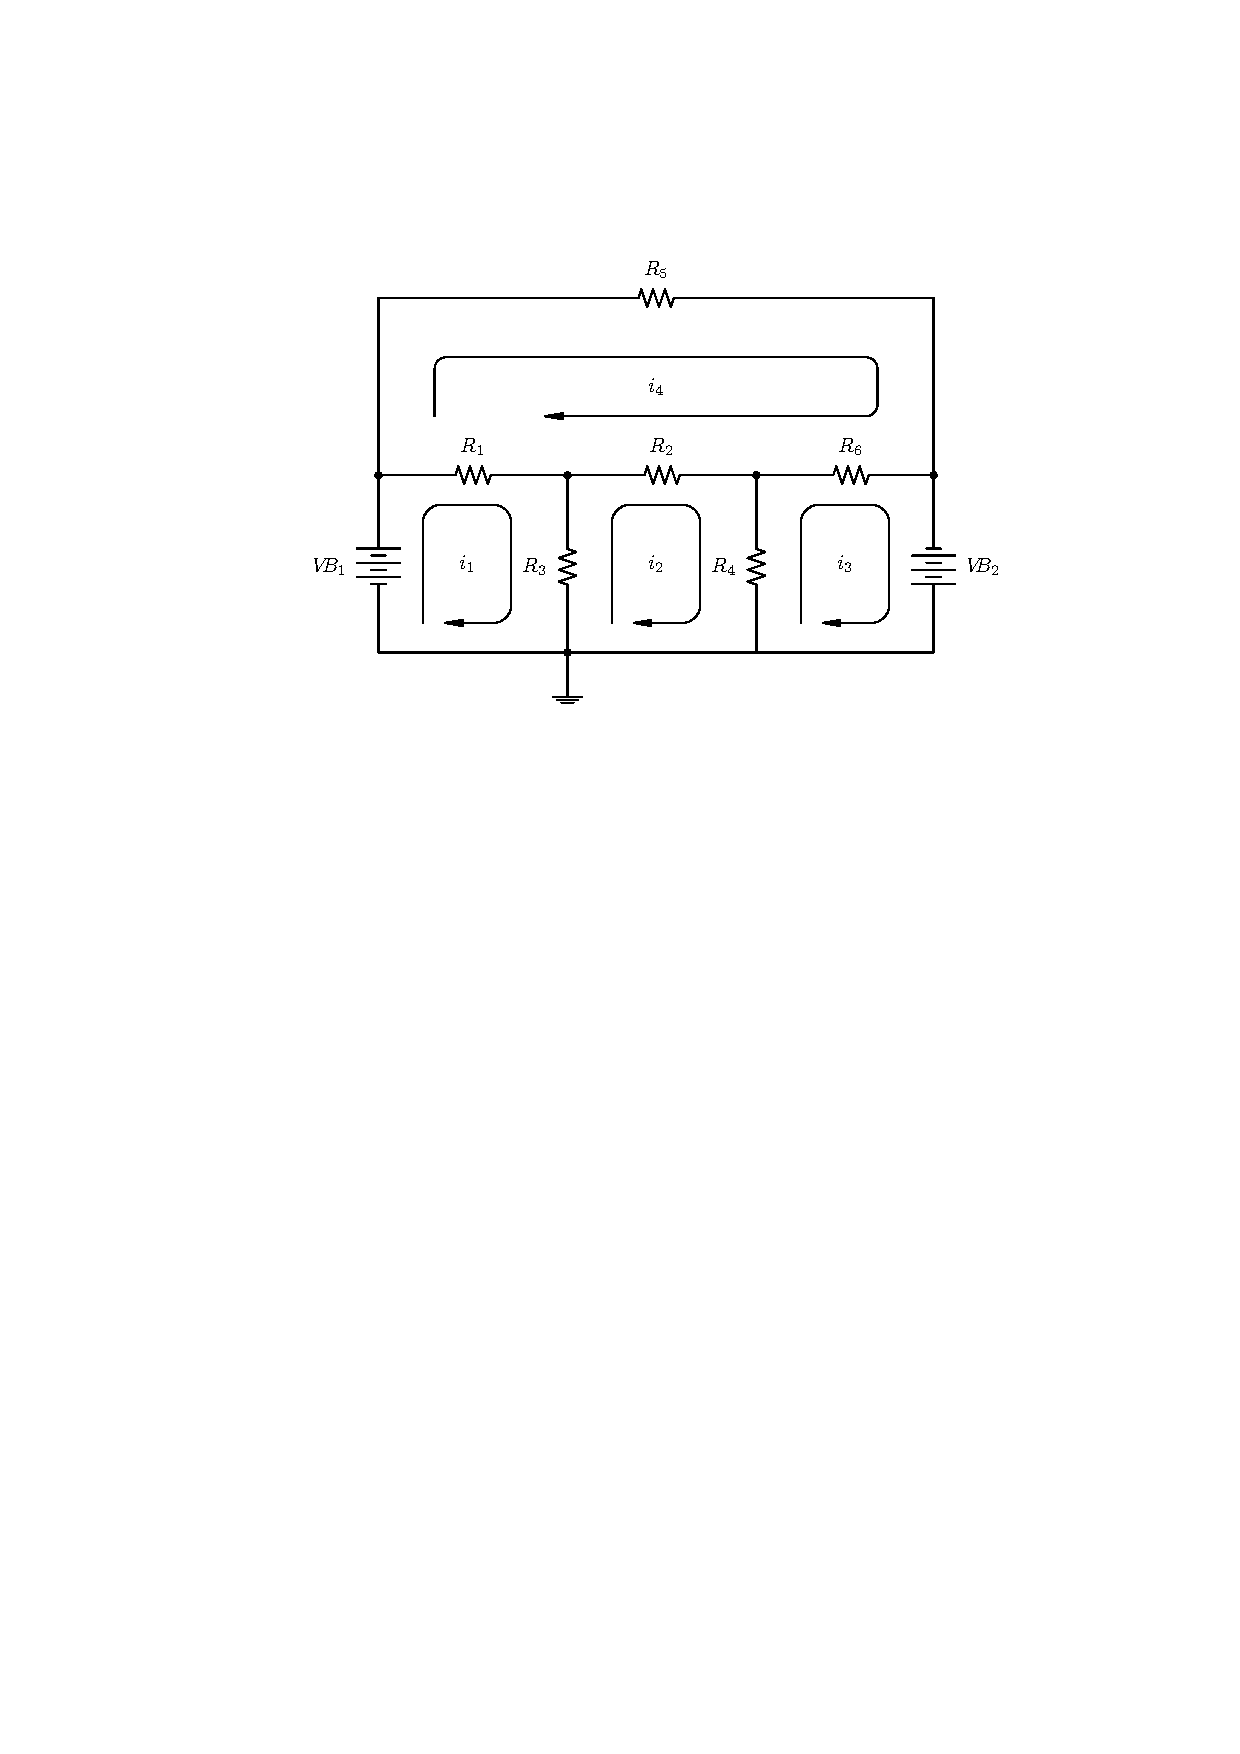
\includegraphics{./MatMethodsGraphics/CircuitDiagram01.pdf}}

The system of linear equations associated with this circuit is

\[ \left\{ \begin{array}{rcl} \left(R_{\mbox{\tiny$1$}} + R_{\mbox{\tiny$3$}}\right)i_{\mbox{\tiny$1$}} - R_{\mbox{\tiny$3$}}i_{\mbox{\tiny$2$}} - R_{\mbox{\tiny$1$}}i_{\mbox{\tiny$4$}} & = & V\!B_{\mbox{\tiny$1$}} \\
-R_{\mbox{\tiny$3$}}i_{\mbox{\tiny$1$}} + \left(R_{\mbox{\tiny$2$}} + R_{\mbox{\tiny$3$}} + R_{\mbox{\tiny$4$}}\right)i_{\mbox{\tiny$2$}} - R_{\mbox{\tiny$4$}}i_{\mbox{\tiny$3$}} - R_{\mbox{\tiny$2$}}i_{\mbox{\tiny$4$}} & = & 0 \\
-R_{\mbox{\tiny$4$}}i_{\mbox{\tiny$2$}} + \left(R_{\mbox{\tiny$4$}} + R_{\mbox{\tiny$6$}}\right)i_{\mbox{\tiny$3$}} - R_{\mbox{\tiny$6$}}i_{\mbox{\tiny$4$}} & = & -V\!B_{\mbox{\tiny$2$}} \\
-R_{\mbox{\tiny$1$}}i_{\mbox{\tiny$1$}} - R_{\mbox{\tiny$2$}}i_{\mbox{\tiny$2$}} - R_{\mbox{\tiny$6$}}i_{\mbox{\tiny$3$}} + \left(R_{\mbox{\tiny$1$}} + R_{\mbox{\tiny$2$}} + R_{\mbox{\tiny$5$}} + R_{\mbox{\tiny$6$}}\right)i_{\mbox{\tiny$4$}} & = & 0 \\  \end{array} \right.\]

Assuming the resistances are all $1 k\Omega$, find the mesh currents if the battery voltages are

\begin{multicols}{2}

\begin{itemize}

\item  $V\!B_{\mbox{\tiny$1$}} = 10 V$ and $V\!B_{\mbox{\tiny$2$}} = 5 V$

\item  $V\!B_{\mbox{\tiny$1$}} = 10 V$ and $V\!B_{\mbox{\tiny$2$}} = 0 V$

\end{itemize}

\end{multicols}

\begin{multicols}{2}

\begin{itemize}

\item  $V\!B_{\mbox{\tiny$1$}} = 0 V$ and $V\!B_{\mbox{\tiny$2$}} = 10 V$

\item  $V\!B_{\mbox{\tiny$1$}} = 10 V$ and $V\!B_{\mbox{\tiny$2$}} = 10 V$

\end{itemize} 

\end{multicols}


{\bf Solution.}  

 Substituting the resistance values into our system of equations, we get

\[ \left\{ \begin{array}{rcl} 2i_{\mbox{\tiny$1$}} - i_{\mbox{\tiny$2$}}-i_{\mbox{\tiny$4$}} & = & V\!B_{\mbox{\tiny$1$}} \\
-i_{\mbox{\tiny$1$}} + 3i_{\mbox{\tiny$2$}} - i_{\mbox{\tiny$3$}} - i_{\mbox{\tiny$4$}} & = & 0 \\
-i_{\mbox{\tiny$2$}} + 2i_{\mbox{\tiny$3$}} - i_{\mbox{\tiny$4$}} & = & -V\!B_{\mbox{\tiny$2$}} \\
-i_{\mbox{\tiny$1$}} - i_{\mbox{\tiny$2$}}-i_{\mbox{\tiny$3$}} + 4i_{\mbox{\tiny$4$}} & = & 0 \\  \end{array} \right.\]
                              
This corresponds to the matrix equation $AX = B$ where 

\[ \begin{array}{ccc} 

A = \left[ \begin{array}{rrrr} 2 & -1 & 0 & -1  \\ -1 & 3 & -1 & -1 \\ 0 & -1 & 2 & -1 \\ -1 & -1 & -1 & 4 \end{array} \right] 

&

 X = \left[ \begin{array}{r} i_{\mbox{\tiny$1$}} \\ i_{\mbox{\tiny$2$}} \\ i_{\mbox{\tiny$3$}} \\ i_{\mbox{\tiny$4$}} \\ \end{array} \right]
 
&

 B = \left[ \begin{array}{r} V\!B_{\mbox{\tiny$1$}} \\ 0 \\ -V\!B_{\mbox{\tiny$2$}} \\ 0 \end{array} \right] 
 \end{array}\]   

When we input the matrix $A$ into the calculator, we find

\begin{center}

\begin{tabular}{cc}

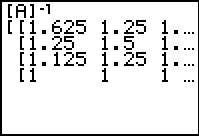
\includegraphics[width=2in]{./MatMethodsGraphics/MATRIXINVERSE01.jpg} &

\hspace{0.75in} 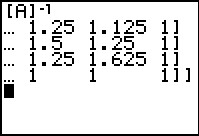
\includegraphics[width=2in]{./MatMethodsGraphics/MATRIXINVERSE02.jpg}  \\

\end{tabular}

\end{center}

from which we have  $A^{-1} = \left[ \begin{array}{rrrr} 1.625 & \hphantom{2}1.25 & 1.125 & \hphantom{2.2}1  \\ 1.25 & 1.5 & 1.25 & 1 \\ 1.125 & 1.25 & 1.625 & 1 \\ 1 & 1 & 1 & 1 \end{array} \right]$. 

To solve the four systems given to us, we find $X=A^{-1}B$ where the value of $B$ is determined by the given values of $V\!B_{\mbox{\tiny$1$}}$ and $V\!B_{\mbox{\tiny$2$}}$

\[\begin{array}{cccc}

 B = \left[ \begin{array}{r} 10 \\ 0 \\ -5 \\ 0 \end{array} \right], & 

 B = \left[ \begin{array}{r} 10 \\ 0 \\ 0 \\ 0 \end{array} \right], & 

B = \left[ \begin{array}{r} 0 \\ 0 \\ -10 \\ 0 \end{array} \right], & 

 B = \left[ \begin{array}{r} 10 \\ 0 \\ 10 \\ 0 \end{array} \right] 

\end{array} \]

\begin{itemize}

\item  For $V\!B_{\mbox{\tiny$1$}} = 10 V$ and $V\!B_{\mbox{\tiny$2$}} = 5 V$, the calculator gives $i_{\mbox{\tiny$1$}} = 10.625 \, \, mA$, $i_{\mbox{\tiny$2$}} = 6.25 \, \, mA$, $i_{\mbox{\tiny$3$}} = 3.125 \, \, mA$, and $i_{\mbox{\tiny$4$}} = 5 \, \, mA$.  We include a calculator screenshot below for this part (and this part only!) for reference.


\centerline{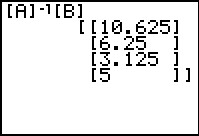
\includegraphics[width=2in]{./MatMethodsGraphics/MATRIXINVERSE03.jpg}}


\item  By keeping  $V\!B_{\mbox{\tiny$1$}} = 10 V$ and setting $V\!B_{\mbox{\tiny$2$}} = 0 V$, we are removing the effect of the second battery. We get $i_{\mbox{\tiny$1$}} = 16.25 \, \, mA$, $i_{\mbox{\tiny$2$}} = 12.5 \, \, mA$, $i_{\mbox{\tiny$3$}} = 11.25 \, \, mA$, and $i_{\mbox{\tiny$4$}} = 10 \, \, mA$.  


\item  Here, we  are zeroing out $V\!B_{\mbox{\tiny$1$}}$ and making $V\!B_{\mbox{\tiny$2$}} = 10$, essentially removing the effect of the first battery.  We find $i_{\mbox{\tiny$1$}} = -11.25 \, \, mA$, $i_{\mbox{\tiny$2$}} = -12.5 \, \, mA$, $i_{\mbox{\tiny$3$}} = -16.25 \, \, mA$, and $i_{\mbox{\tiny$4$}} = -10 \, \, mA$, where the negatives indicate that the current is flowing in the opposite direction as is indicated on the diagram. The reader is encouraged to study the symmetry here, and if need be, hold up a mirror to the diagram to literally `see' what is happening.

\item  For $V\!B_{\mbox{\tiny$1$}} = 10 V$ and $V\!B_{\mbox{\tiny$2$}} = 10 V$, we get $i_{\mbox{\tiny$1$}} = 5 \, \, mA$, $i_{\mbox{\tiny$2$}} = 0 \, \, mA$, $i_{\mbox{\tiny$3$}} = -5 \, \, mA$, and $i_{\mbox{\tiny$4$}} = 0 \, \, mA$.  The mesh currents $i_{\mbox{\tiny$2$}}$ and $i_{\mbox{\tiny$4$}}$ being zero is a consequence of both batteries `pushing' in equal but opposite directions, causing the net flow of electrons in these two regions to cancel out. \qed

\end{itemize}

\end{ex}

\subsection{Exercises}

\label{ExercisesforMatMethods}

In Exercises \ref{findmatinversefirst} - \ref{findmatinverselast}, find the inverse of the matrix or state that the matrix is not invertible.

\begin{multicols}{2}
\begin{enumerate}

\item $A = \left[ \begin{array}{rr} 1 & 2 \\ 3 & 4 \end{array} \right]$ \label{findmatinversefirst}
\item $B = \left[ \begin{array}{rr} 12 & -7 \\ -5 & 3 \end{array} \right]$ \label{matrixB}

\setcounter{HW}{\value{enumi}}
\end{enumerate}
\end{multicols}

\begin{multicols}{2}
\begin{enumerate}
\setcounter{enumi}{\value{HW}}

\item $C = \left[ \begin{array}{rr} 6 & 15 \\ 14 & 35 \end{array} \right]$
\item $D = \left[ \begin{array}{rr} 2 & -1 \\ 16 & -9 \end{array} \right]$ \label{matrixD}

\setcounter{HW}{\value{enumi}}
\end{enumerate}
\end{multicols}

\begin{multicols}{2}
\begin{enumerate}
\setcounter{enumi}{\value{HW}}

\item $E = \left[ \begin{array}{rrr} 3 & 0 & 4 \\ 2 & -1 & 3 \\ -3 & 2 & -5 \end{array} \right]$ \label{matrixE}
\item $F = \left[ \begin{array}{rrr} 4 & \hphantom{-}6 & -3 \\ 3 & 4 & -3 \\ 1 & 2 & 6 \end{array} \right]$

\setcounter{HW}{\value{enumi}}
\end{enumerate}
\end{multicols}

\begin{multicols}{2}
\begin{enumerate}
\setcounter{enumi}{\value{HW}}

\item $G = \left[ \begin{array}{rrr} 1 & \hphantom{1}2 & 3 \\ 2 & 3 & 11 \\ 3 & 4 & 19 \end{array} \right]$
\item $H = \left[ \begin{array}{rrrr} 1 & 0 & -3 & \hphantom{-}0 \\ 2 & -2 & 8 & 7 \\ -5 & 0 & 16 & 0 \\ 1 & 0 & 4 & 1 \end{array} \right]$ \label{findmatinverselast}

\setcounter{HW}{\value{enumi}}
\end{enumerate}
\end{multicols}


In Exercises \ref{2by2inversefirst} - \ref{2by2inverselast}, use one matrix inverse to solve the following systems of linear equations.

\begin{multicols}{3}
\begin{enumerate}
\setcounter{enumi}{\value{HW}}

\item $\left\{ \begin{array}{rcr}   3x + 7y & = & 26 \\ 5x + 12y & = & 39  \end{array} \right.$ \label{2by2inversefirst}
\item $\left\{ \begin{array}{rcr}   3x + 7y & = &  0 \\ 5x + 12y & = & -1  \end{array} \right.$
\item $\left\{ \begin{array}{rcr}   3x + 7y & = & -7 \\ 5x + 12y & = &  5  \end{array} \right.$ \label{2by2inverselast}


\setcounter{HW}{\value{enumi}}
\end{enumerate}
\end{multicols}


In Exercises \ref{3by3inversefirst} - \ref{3by3inverselast}, use the inverse of $E$ from Exercise \ref{matrixE} above to solve the following systems of linear equations.

\begin{multicols}{3}
\begin{enumerate}
\setcounter{enumi}{\value{HW}}

\item $\left\{ \begin{array}{rcr}   3x + 4z & = & 1 \\ 2x - y + 3z & = & 0 \\ \!-3x + 2y - 5z & = & 0  \end{array} \right.$ \label{3by3inversefirst}
\item $\left\{ \begin{array}{rcr}   3x + 4z & = & 0 \\ 2x - y + 3z & = & 1 \\ \!-3x + 2y - 5z & = & 0  \end{array} \right.$
\item $\left\{ \begin{array}{rcr}   3x + 4z & = & 0 \\ 2x - y + 3z & = & 0 \\ \!-3x + 2y - 5z & = & 1  \end{array} \right.$ \label{3by3inverselast}

\setcounter{HW}{\value{enumi}}
\end{enumerate}
\end{multicols}

\begin{enumerate}
\setcounter{enumi}{\value{HW}}

\item  This exercise is a continuation of Example \ref{rotationmatrixex} in Section \ref{MatArithmetic} and gives another application of matrix inverses.  Recall that given the position matrix $P$ for a point in the plane, the matrix $RP$ corresponds to a point rotated $45^{\circ}$ counterclockwise from $P$ where
 
\[R = \left[ \begin{array}{rr} \frac{\sqrt{2}}{2} & -\frac{\sqrt{2}}{2} \\[3pt] \frac{\sqrt{2}}{2} & \frac{\sqrt{2}}{2} \\ \end{array} \right]\]
 
\begin{enumerate}

\item  Find $R^{-1}$.
\item  If $RP$ rotates a point counterclockwise $45^{\circ}$, what should $R^{-1}P$ do?  Check your answer by finding $R^{-1}P$ for various points on the coordinate axes and the lines $y=\pm x$.
\item  Find $R^{-1}P$ where $P$ corresponds to a generic point $P(x,y)$. Verify that this takes points on the curve $y=\frac{2}{x}$ to points on the curve $x^2-y^2=4$.

\end{enumerate}

\item \label{SasquatchDiet} A Sasquatch's diet consists of three primary foods:  Ippizuti Fish, Misty Mushrooms, and Sun Berries.  Each serving of Ippizuti Fish is 500 calories, contains 40 grams of protein, and has no Vitamin X.  Each serving of Misty Mushrooms is 50 calories, contains 1 gram of protein, and 5 milligrams of Vitamin X.  Finally, each serving of Sun Berries is 80 calories, contains no protein, but has 15 milligrams of Vitamin X.\footnote{Misty Mushrooms and Sun Berries are the only known fictional sources of Vitamin X.}

\begin{enumerate}

\item  If an adult male Sasquatch requires 3200 calories, 130 grams of protein, and 275 milligrams of Vitamin X daily, use a matrix inverse to find how many servings each of Ippizuti Fish, Misty Mushrooms, and Sun Berries he needs to eat each day.

\item  An adult female Sasquatch requires 3100 calories, 120 grams of protein, and 300 milligrams of Vitamin X daily. Use the matrix inverse you found in part (a) to find how many servings each of Ippizuti Fish, Misty Mushrooms, and Sun Berries she needs to eat each day.

\item  An adolescent Sasquatch requires 5000 calories, 400 grams of protein daily, but no Vitamin X daily.\footnote{Vitamin X is needed to sustain Sasquatch longevity only.}   Use the matrix inverse you found in part (a) to find how many servings each of Ippizuti Fish, Misty Mushrooms, and Sun Berries she needs to eat each day.

\end{enumerate}


\item Matrices can be used in cryptography.  Suppose we wish to encode the message `BIGFOOT LIVES'.  We start by assigning a number to each letter of the alphabet, say $A=1$, $B=2$ and so on.  We reserve $0$ to act as a space.  Hence, our message `BIGFOOT LIVES' corresponds to the string of numbers `2, 9, 7, 6, 15, 15, 20, 0, 12, 9, 22, 5, 19.' To encode this message, we use an invertible matrix.  Any invertible matrix will do, but for this exercise, we choose

\[ A = \left[ \begin{array}{rrr} 2 & -3 & 5 \\ 3 & 1 &-2 \\ -7 & 1 & -1 \end{array} \right] \]

Since $A$ is  $3 \times 3$ matrix, we encode our message string into a matrix $M$ with $3$ rows.  To do this, we take the first three numbers, 2 9 7, and make them our first column, the next three numbers, 6 15 15, and make them our second column, and so on.  We put $0$'s to round out the matrix.


\[ M = \left[  \begin{array}{rrrrr} 2 & 6 & 20 & 9 & 19 \\ 9 & 15 & 0 & 22 & 0 \\ 7 & 15 & 12 & 5 & 0 \end{array} \right] \]

To encode the message, we find the product $AM$

\[AM =  \left[ \begin{array}{rrr} 2 & -3 & 5 \\ 3 & 1 &-2 \\ -7 & 1 & -1 \end{array} \right]\left[  \begin{array}{rrrrr} 2 & 6 & 20 & 9 & 19 \\ 9 & 15 & 0 & 22 & 0 \\ 7 & 15 & 12 & 5 & 0 \end{array} \right] = \left[  \begin{array}{rrrrr} 12 & 42 & 100 & -23 & 38 \\ 1 & 3 & 36 & 39 & 57 \\ -12 & -42 & -152 & -46 & -133 \end{array} \right]\]

So our coded message is `12, 1, $-12$, 42, 3, $-42$, 100, 36, $-152$, $-23$, 39, $-46$, 38, 57, $-133$.'  To decode this message, we start with this string of numbers, construct a message matrix as we did earlier (we should get the matrix $AM$ again) and then multiply by $A^{-1}$.

\begin{enumerate}

\item  Find $A^{-1}$.

\item  Use $A^{-1}$ to decode the message and check this method actually works.

\item  Decode the message `14, 37, $-76$, 128, 21, $-151$, 31, 65, $-140$'

\item  Choose another invertible matrix and encode and decode your own messages.

\end{enumerate}

\item Using the matrices $A$ from Exercise \ref{findmatinversefirst}, $B$ from Exercise \ref{matrixB} and $D$ from Exercise \ref{matrixD}, show $AB = D$ and  $D^{-1} = B^{-1}A^{-1}$.  That is, show that $(AB)^{-1} = B^{-1}A^{-1}$. 

\item Let $M$ and $N$ be invertible $n \times n$ matrices.  Show that $(MN)^{-1} = N^{-1}M^{-1}$ and compare your work to Exercise \ref{fcircginverse} in Section \ref{InverseFunctions}.


\end{enumerate}

\newpage

\subsection{Answers}

\begin{multicols}{2} 
\begin{enumerate}


\item $A^{-1} = \left[ \begin{array}{rr} -2 & 1 \\[3pt] \frac{3}{2} & -\frac{1}{2} \end{array} \right]$
\item $B^{-1} = \left[ \begin{array}{rr} 3 & 7 \\ 5 & 12 \end{array} \right]$

\setcounter{HW}{\value{enumi}}
\end{enumerate}
\end{multicols}

\begin{multicols}{2} 
\begin{enumerate}
\setcounter{enumi}{\value{HW}}

\item $C \vphantom{\left[ \begin{array}{rr} \frac{9}{2} & -\frac{1}{2} \\ 8 & -1 \end{array} \right]}$ is not invertible
\item $D^{-1} = \left[ \begin{array}{rr} \frac{9}{2} & -\frac{1}{2} \\ 8 & -1 \end{array} \right]$

\setcounter{HW}{\value{enumi}}
\end{enumerate}
\end{multicols}

\begin{multicols}{2} 
\begin{enumerate}
\setcounter{enumi}{\value{HW}}

\item $E^{-1} = \left[ \begin{array}{rrr} -1 & 8 & 4 \\ 1 & -3 & -1 \\ 1 & -6 & -3 \end{array} \right] \vphantom{\left[ \begin{array}{rrr} -\frac{5}{2} & \frac{7}{2} & \frac{1}{2} \\[3pt] \frac{7}{4} & -\frac{9}{4} & -\frac{1}{4} \\[3pt] -\frac{1}{6} & \frac{1}{6} & \frac{1}{6} \end{array} \right]}$
\item $F^{-1} = \left[ \begin{array}{rrr} -\frac{5}{2} & \frac{7}{2} & \frac{1}{2} \\[3pt] \frac{7}{4} & -\frac{9}{4} & -\frac{1}{4} \\[3pt] -\frac{1}{6} & \frac{1}{6} & \frac{1}{6} \end{array} \right]$

\setcounter{HW}{\value{enumi}}
\end{enumerate}
\end{multicols}

\begin{multicols}{2} 
\begin{enumerate}
\setcounter{enumi}{\value{HW}}

\item $G \vphantom{\left[ \begin{array}{rrrr} 16 & 0 & 3 & 0 \\[3pt] -90 & -\frac{1}{2} & -\frac{35}{2} & \frac{7}{2} \\[3pt] 5 & 0 & 1 & 0 \\[3pt] -36 & 0 & -7 & \hphantom{-}1 \end{array} \right]}$ is not invertible
\item $H^{-1} = \left[ \begin{array}{rrrr} 16 & 0 & 3 & 0 \\[3pt] -90 & -\frac{1}{2} & -\frac{35}{2} & \frac{7}{2} \\[3pt] 5 & 0 & 1 & 0 \\[3pt] -36 & 0 & -7 & \hphantom{-}1 \end{array} \right]$

\setcounter{HW}{\value{enumi}}
\end{enumerate}
\end{multicols}

The coefficient matrix is $B^{-1}$ from Exercise \ref{matrixB} above so the inverse we need is $(B^{-1})^{-1} = B$. 

\begin{enumerate}
\setcounter{enumi}{\value{HW}}

\item $\left[ \begin{array}{rr} 12 & -7 \\ -5 & 3 \end{array} \right] \left[ \begin{array}{r} 26 \\ 39 \end{array} \right] = \left[ \begin{array}{r} 39 \\ -13 \end{array} \right] \;$ So $x = 39$ and $y = -13$.
\item $\left[ \begin{array}{rr} 12 & -7 \\ -5 & 3 \end{array} \right] \left[ \begin{array}{r} 0 \\ -1 \end{array} \right] = \left[ \begin{array}{r} 7 \\ -3 \end{array} \right] \;$ So $x = 7$ and $y = -3$.
\item $\left[ \begin{array}{rr} 12 & -7 \\ -5 & 3 \end{array} \right] \left[ \begin{array}{r} -7 \\ 5 \end{array} \right] = \left[ \begin{array}{r} -119 \\ 50 \end{array} \right] \;$ So $x = -119$ and $y = 50$.

\setcounter{HW}{\value{enumi}}
\end{enumerate}

The coefficient matrix is $E = \left[ \begin{array}{rrr} 3 & 0 & 4 \\ 2 & -1 & 3 \\ -3 & 2 & -5 \end{array} \right]$ from Exercise \ref{matrixE}, so $E^{-1} = \left[ \begin{array}{rrr} -1 & 8 & 4 \\ 1 & -3 & -1 \\ 1 & -6 & -3 \end{array} \right]$ 

\begin{enumerate}
\setcounter{enumi}{\value{HW}}

\item $\left[ \begin{array}{rrr} -1 & 8 & 4 \\ 1 & -3 & -1 \\ 1 & -6 & -3 \end{array} \right] \left[ \begin{array}{r} 1 \\ 0 \\ 0 \end{array} \right] = \left[ \begin{array}{r} -1 \\ 1 \\ 1 \end{array} \right] \;$ So $x = -1$, $y = 1$ and $z = 1$.
\item $\left[ \begin{array}{rrr} -1 & 8 & 4 \\ 1 & -3 & -1 \\ 1 & -6 & -3 \end{array} \right] \left[ \begin{array}{r} 0 \\ 1 \\ 0 \end{array} \right] = \left[ \begin{array}{r} 8 \\ -3 \\ -6 \end{array} \right] \;$ So $x = 8$, $y = -3$ and $z = -6$.
\item $\left[ \begin{array}{rrr} -1 & 8 & 4 \\ 1 & -3 & -1 \\ 1 & -6 & -3 \end{array} \right] \left[ \begin{array}{r} 0 \\ 0 \\ 1 \end{array} \right] = \left[ \begin{array}{r} 4 \\ -1 \\ -3 \end{array} \right] \;$ So $x = 4$, $y = -1$ and $z = -3$.

\setcounter{HW}{\value{enumi}}
\end{enumerate}

\begin{enumerate}
\setcounter{enumi}{\value{HW}}

\addtocounter{enumi}{1}

\item  \begin{enumerate} \item  The adult male Sasquatch needs:  3 servings of Ippizuti Fish, 10 servings of Misty Mushrooms, and 15 servings of Sun Berries daily.

\item  The adult female Sasquatch needs:  3 servings of Ippizuti Fish and 20 servings of Sun Berries daily.  (No Misty Mushrooms are needed!)

\item  The adolescent Sasquatch requires 10 servings of Ippizuti Fish daily.  (No Misty Mushrooms or Sun Berries are needed!)

\end{enumerate}

\item  \begin{enumerate}

\item  $A^{-1} = \left[ \begin{array}{rrr} 1 & 2 & 1 \\ 17 & 33 & 19 \\ 10 & 19 & 11 \end{array} \right] $

\item  $ \left[ \begin{array}{rrr} 1 & 2 & 1 \\ 17 & 33 & 19 \\ 10 & 19 & 11 \end{array} \right] \left[  \begin{array}{rrrrr} 12 & 42 & 100 & -23 & 38 \\ 1 & 3 & 36 & 39 & 57 \\ -12 & -42 & -152 & -46 & -133 \end{array} \right] =  \left[  \begin{array}{rrrrr} 2 & 6 & 20 & 9 & 19 \\ 9 & 15 & 0 & 22 & 0 \\ 7 & 15 & 12 & 5 & 0 \end{array} \right] \quad \checkmark$

\item  `LOGS RULE'

\end{enumerate}

\end{enumerate}

\closegraphsfile